\documentclass[11pt]{article}
\usepackage[paper=a4paper,margin=2cm]{geometry}
\usepackage[svgnames]{xcolor}
\usepackage{listings}
\usepackage{sourcecodepro}
\usepackage{graphicx}

\graphicspath{ {./images/} }

\lstset{
    language=R,
    basicstyle=\footnotesize\ttfamily,
    stringstyle=\color{DarkGreen},
    commentstyle=\color{DarkBlue},
    keywordstyle=\footnotesize\ttfamily,
    showstringspaces=false,
    deletekeywords={/},
    xleftmargin=.35em,
    xrightmargin=.35em,
}

\begin{document}

\section*{Pergunta 3}

\begin{lstlisting}
    library(ggplot2)
    theme_set(theme_light())

    dados <- readxl::read_xlsx("./data/electricity.xlsx")
    tipo <- "Renewables"
    ano <- 2015
    paises <- c("IEA Total", "Hungary", "Iceland")

    dados <- dados[dados$YEAR >= ano & 
                   dados$COUNTRY %in% paises & 
                   dados$PRODUCT == tipo,]
    dados$share <- as.numeric(dados$share) * 100
    dados$tempo <- as.Date(paste(dados$YEAR, dados$MONTH, "01", sep = "-"))

    ggplot(dados) +
    geom_line(aes(x = tempo, y = share, colour = COUNTRY)) +
    ylim(0, 100) +
    labs(title = paste("Evolution of the share of", tipo),
         subtitle = paste("Relative to other energy sources, from", ano),
         y = "Share (%)",
         x = "Time")
\end{lstlisting}

\vspace{14pt}

\begin{center}
    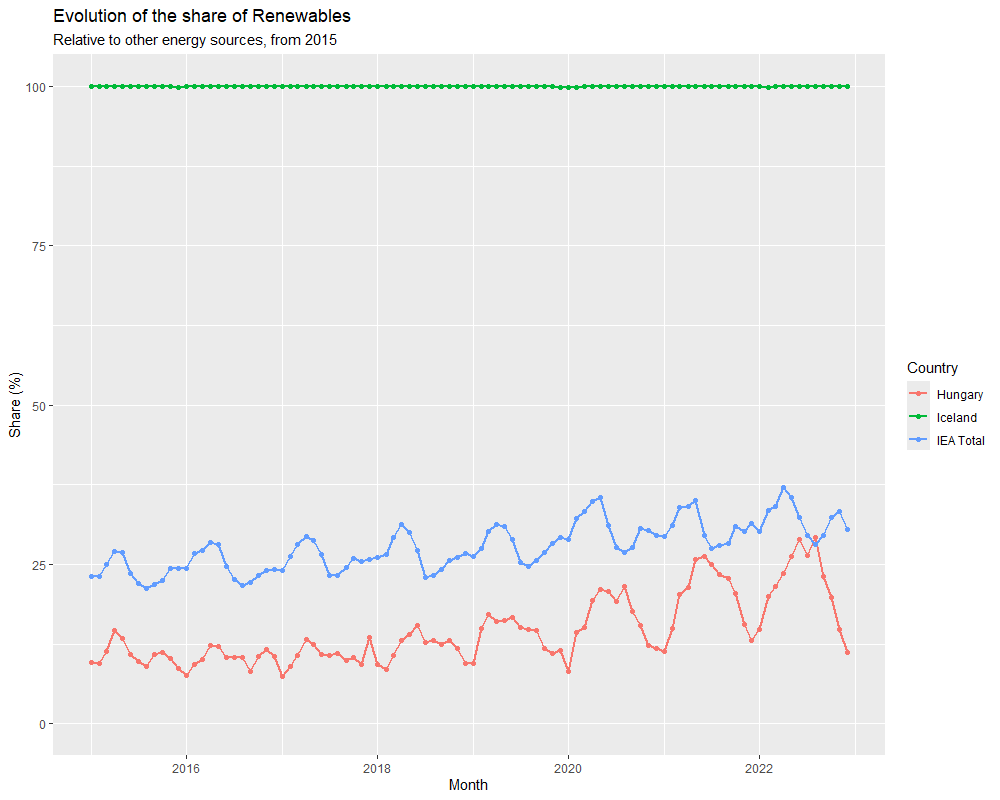
\includegraphics[width=\linewidth]{pergunta_3.png}
\end{center}

\end{document}